\section{$H \rightarrow WW$ Analyse}

In diesem Versuchsteil soll die Existenz des Higgs-Bosons überprüft werden.
Dafür müssen wir zuerst vermutete Higgs-Ereignisse innerhalb unserer Daten finden.
Diese sind jedoch relativ selten, weshalb wir einen großen Untergrund haben.
Die erste Aufgabe bestand daher darin, Cuts aus physikalischen Überlegungen herzuleiten und zu implementieren, die Higgs-Ereignisse vom Untergrund trennen.

Zum Testen von Cuts stand uns die Seite \url{http://opendata.atlas.cern/visualisations/analyser-js.php} zur Verfügung.
Diese enthalt eine Mischung aus simulierten und realen ATLAS-Daten, innerhalb derer wir Cuts implementieren und deren Auswirkungen testen können.
Die dortigen Daten enthalten neben den gewünschten $H \rightarrow WW$ Ereignissen noch einen Untergrund aus $WW$, $t\overline{t}$ und $Z$ Ereignissen.
In Abb. \ref{test_nocuts} sind die Ereignisse ohne Cuts zu sehen.


\begin{figure}[h]
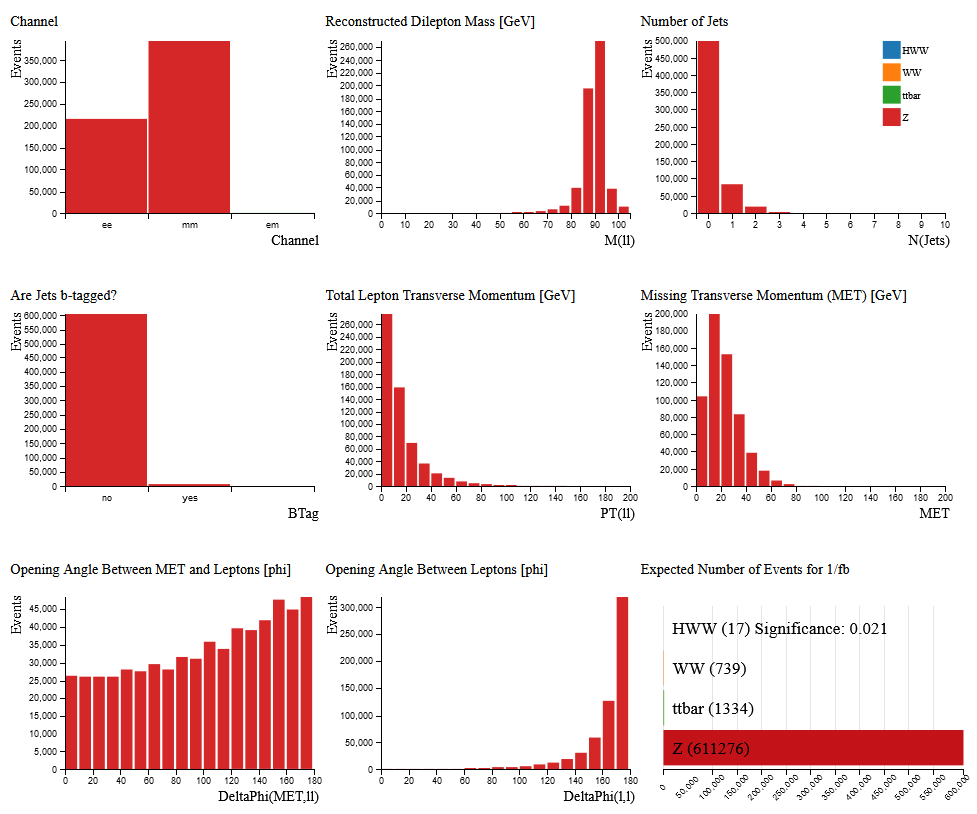
\includegraphics[width=\linewidth]{../Pictures/Auswertung/test_nocuts.png}
\caption{Daten ohne Cuts \cite{opendata}}
\label{test_nocuts}
\end{figure}

\clearpage

Wie zu sehen ist, werden diese Daten von einem riesigen $Z$ Untergrund dominiert.
Auf 17 $H$ Ereignisse kommen hier 611.276 $Z$ Ereignisse, was die Notwendigkeit von Cuts noch einmal verdeutlicht.
Andere Untergrundereignisse die hier betrachtet werden, sind $t\overline{t}$ (1443) und $WW$ (739) Ereignisse.
Als Maß für die Qualität unserer Cuts betrachten wir im Folgenden die Signifikanz der Higgs-Ereignisse, die ohne Cuts bei 0,021 liegt.

Für die ersten Cuts rekapitulieren wir wieder die Zerfallskanäle:
Das Z-Boson zerfällt bevorzugt in ein Lepton-Antilepton-Paar oder auf hadronischem Weg.
Dabei werden zwei gleiche Leptonen ($ee$ oder $\mu \mu$) als Endprodukt verbleiben.
Beim Zerfall zweier W-Bosonen können gemischte Endzustände ($e \mu$) existieren.
Ein Cut der nur gemischte Endzustände betrachtet, sollte also einen guten Anteil des Z-Untergrunds beseitigen (siehe Channel in Abb. \ref{test_firstcuts}).
Zusätzlich sollte der Endzustand genauso wie wie der Endzustand elektrisch Neutral sein, was innerhalb dieser Daten nicht von Relevanz ist, aber später genutzt wird.
Das Ergebnis dieses ersten Cuts ist in Abb. \ref{mixed} zu sehen.
Die ausgegrauten Ereignisse wurden hier gecutted.

\begin{figure}[h]
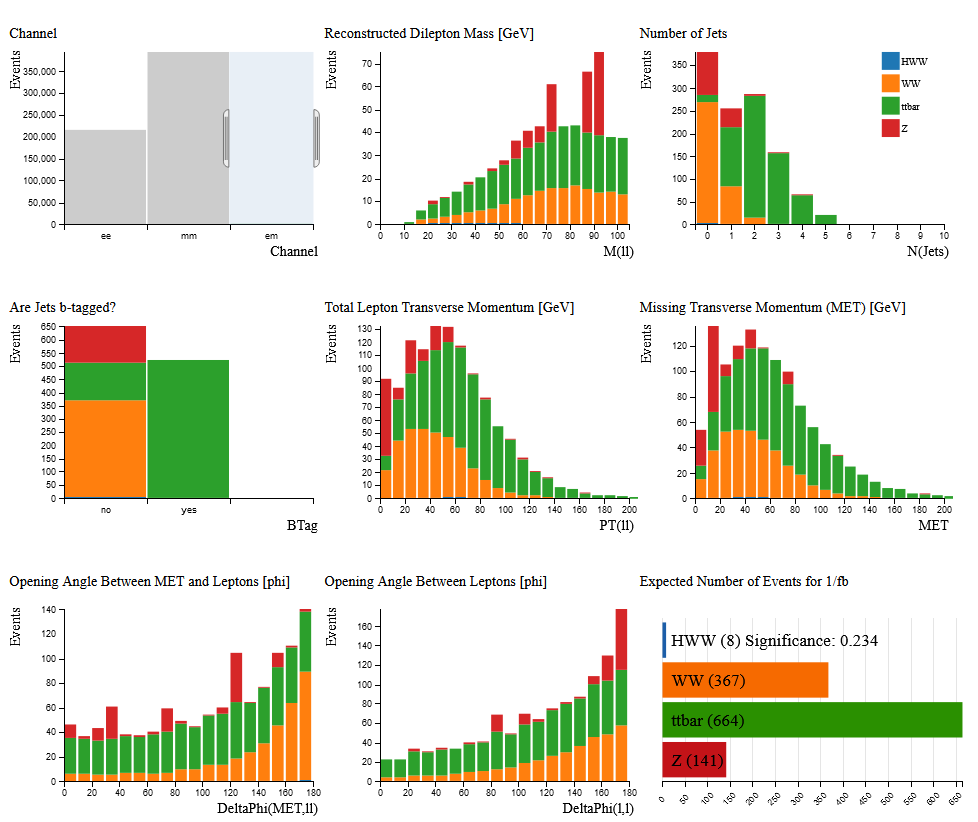
\includegraphics[width=\linewidth]{../Pictures/Auswertung/mixed.png}
\caption{Nur gemischte Leptonen \cite{opendata}}
\label{mixed}
\end{figure}

\clearpage

Wie wir sehen können, wurde der Z-Untergrund massiv reduziert.
Ebenfalls ein sinnvoller erster Cut würde darin bestehen, b-Jets zu ignorieren, da diese vor allem von $t\overline{t}$ Ereignissen stammen sollten.
Da wir die Masse des Higgs-Bosons ($125$ GeV) bereits kennen bietet es sich auch an Cuts an die invariante Leptonenmasse zu legen.
Hier ist jetzt jedoch zu beachten, dass bei gemischten Leptonenereignissen Neutrinos entstanden sein müssen, die nicht im Detektor gemessen werden können.
Deshalb sollte die invariante Masse niedriger als die bekannte Higgs-Masse angesetzt werden.

Ein Ergebnis dieser beschriebenen Cuts ist in Abb. \ref{test_firstcuts} zu sehen.

\begin{figure}[h]
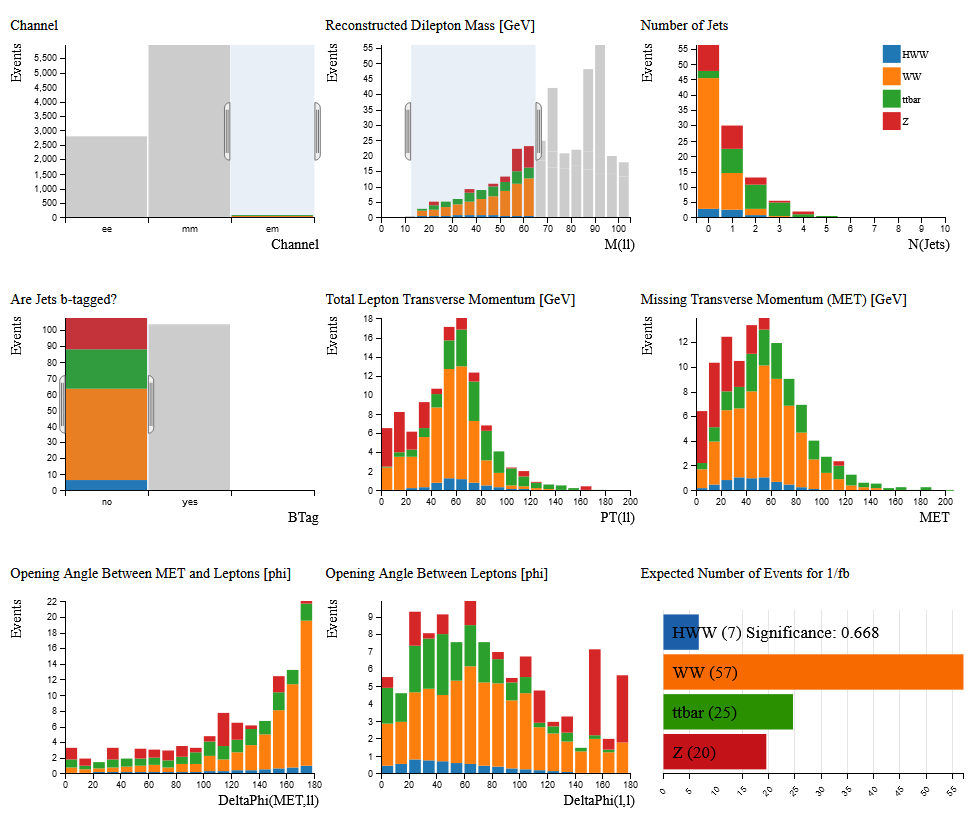
\includegraphics[width=\linewidth]{../Pictures/Auswertung/test_firstcuts.png}
\caption{Daten mit ersten Cuts \cite{opendata}}
\label{test_firstcuts}
\end{figure}

Als Ergebnis dieser ersten Cuts können wir sehen, dass der $Z$-Untergrund wesentlich reduziert wurde, auf nur noch 20 Ereignisse.
Gleichzeitig haben wir zwar auch 10 unserer Higgs-Ereignisse verloren, die Signifikanz hat sich jedoch aufgrund des reduzierten Untergrunds auf 0,668 erhöht.
Der Restuntergrund wird vor allem von 57 $WW$-Ereignissen dominiert.
Diese sollten von Natur aus recht schwer von $H \rightarrow WW$ Ereignisse zu trennen sein.
Weitere Cuts die angesetzt wurden, zielten darauf aus höhere fehlende transversale Energien, höhere Jet-zahlen oder niedrige Winkel zwischen den Leptonen zu reduzieren.
Dies alles hatte jedoch nur noch kleinere Auswirkungen, mit weiteren Cuts war nur noch eine Steigerung der Signifikanz auf 0,743 möglich (siehe Abb. \ref{test_secondcuts}.
Mit Blick auf die Daten ist eine weitere Erhöhung der Signifikanz scheinbar nicht möglich.

Zusammenfassend haben wir also von Ursprünglich über 600.000 Ereignissen, unter denen sich 17 Higgs-Ereignisse mit einer Signifikanz von 0,021 befanden, nach Implementierung der Cuts noch 37 mit 4 Higgs-Ereignissen, die jetzt jedoch eine Signifikanz von 0,743 besitzen.
Der verbliebende Untergrund besteht 24 $WW$, 9 $t\overline{t}$.
Der $Z$-Untergrund konnte vollständig beseitigt werden.
Eine vollständige Beseitigung des $WW$ Untergrundes erscheint ohne weitere Berechnungen nicht realistisch, aufgrund der Ähnlichkeit zum $H \rightarrow WW$.
Möglicherweise wäre jedoch noch mit besseren Cuts eine komplette Beseitigung der $t\overline{t}$ Ereignisse möglich.

\begin{figure}[h]
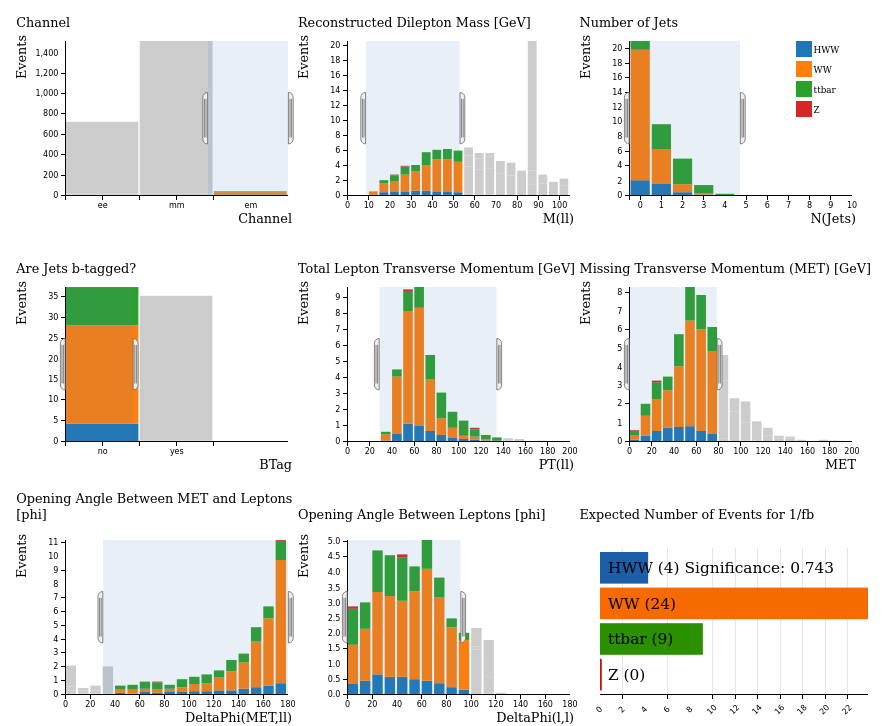
\includegraphics[width=\linewidth]{../Pictures/Auswertung/test_secondcuts.png}
\caption{Finale Cuts \cite{opendata}}
\label{test_secondcuts}
\end{figure}

\clearpage

Die so getesteten Cuts wurden im Folgenden auf die uns zur Verfügung stehenden Daten angewandt.
Als Maß nutzen wir nun keine Signifikanz, sondern das Verhältnis von Signal zum Untergrund (S/B in den Abbildungen) sowie von Daten und Simulation (Data/MC in den Abbildungen).
In Abb. \ref{Cuts_mass} und \ref{Cuts_momentum} werden die Auswirkungen dieser Cuts schrittweise dargestellt.
Zur Anschaulichkeit beschränken wir uns in der Darstellung auf die invariante Masse und den Impuls der Leptonen, die anderen Größen wurden jedoch außerhalb des Protokolls auch im Auge behalten.
Auch hier scheinen unsere Cuts den Untergrund effektiv zu reduzieren.
Das Verhältnis zwischen Daten und Simulation konnte ebenfalls in dem Bereich in dem Higgs-Bosonen auftreten auf Werte nahe 1 gebracht werden, wobei dieses außerhalb der Bereiche schnell deutlich schlechtere Werte annimmt.
Zu beobachten ist ebenfalls, dass der Fehler innerhalb der Daten sich mit Anzahl der Cuts erhöht, was jedoch zu erwarten ist.

\begin{figure}[h]
\begin{subfigure}{.5\textwidth}
\centering
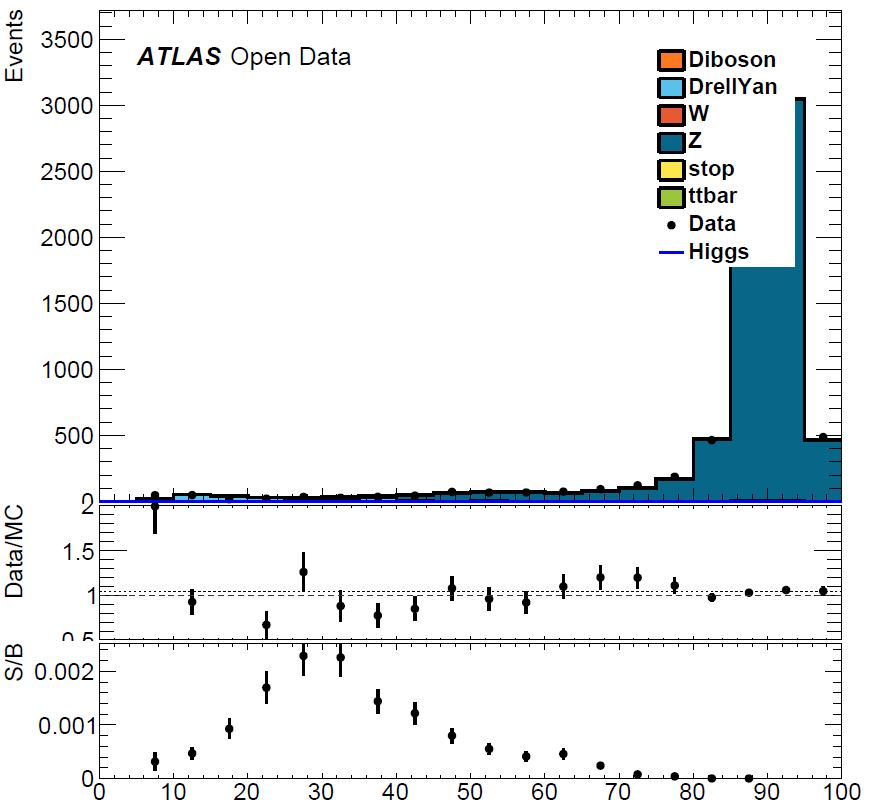
\includegraphics[width=.8\linewidth]{../Pictures/Auswertung/nocuts_mass.png}
\caption{Daten ohne Cuts}
\end{subfigure}%
\begin{subfigure}{.5\textwidth}
\centering
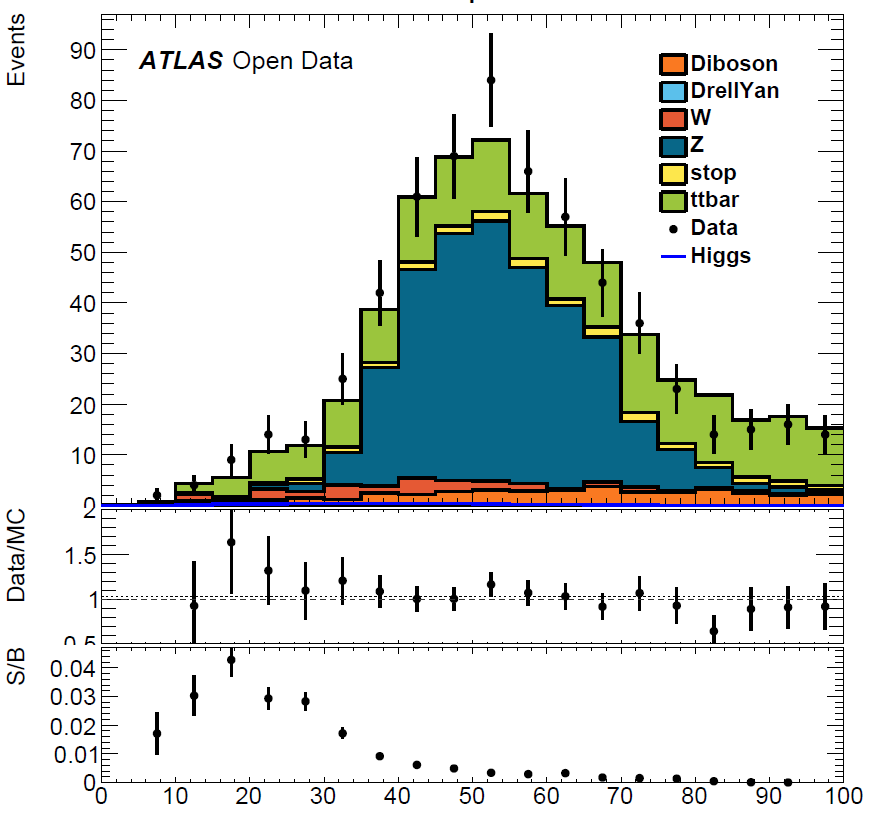
\includegraphics[width=.8\linewidth]{../Pictures/Auswertung/1cut_mass.png}
\caption{Nur gemischte Leptonen und kein Ladungsüberschuss}
\end{subfigure}%
\vskip\baselineskip
\begin{subfigure}{.5\textwidth}
\centering
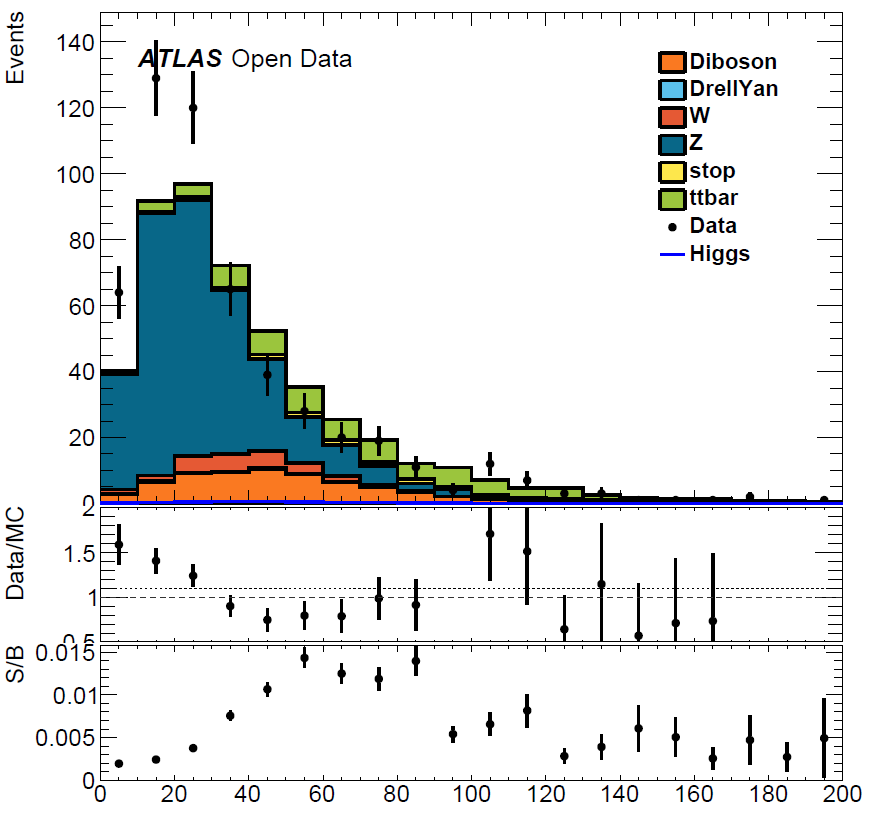
\includegraphics[width=.8\linewidth]{../Pictures/Auswertung/2cut_mass.png}
\caption{Cut aller b-Jets}
\end{subfigure}%
\begin{subfigure}{.5\textwidth}
\centering
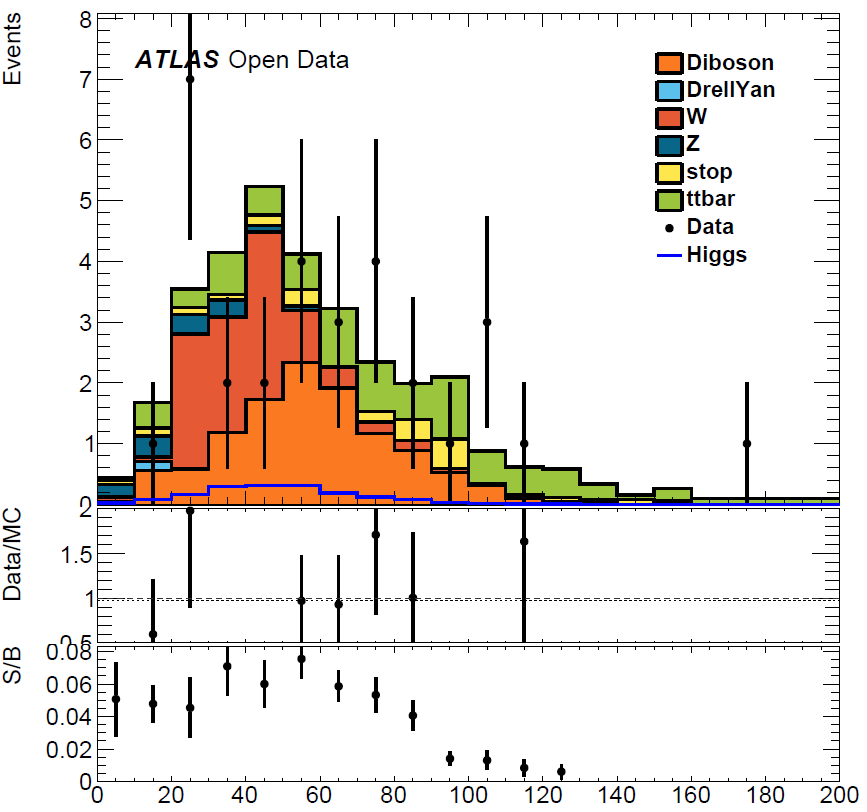
\includegraphics[width=.8\linewidth]{../Pictures/Auswertung/3cut_mass.png}
\caption{weitere Cuts}
\end{subfigure}%
\caption{Auswirkungen der Cuts auf die Ereignisse unter Betrachtung der invarianten Masse}
\label{Cuts_mass}
\end{figure}

\begin{figure}[h]
\begin{subfigure}{.5\textwidth}
\centering
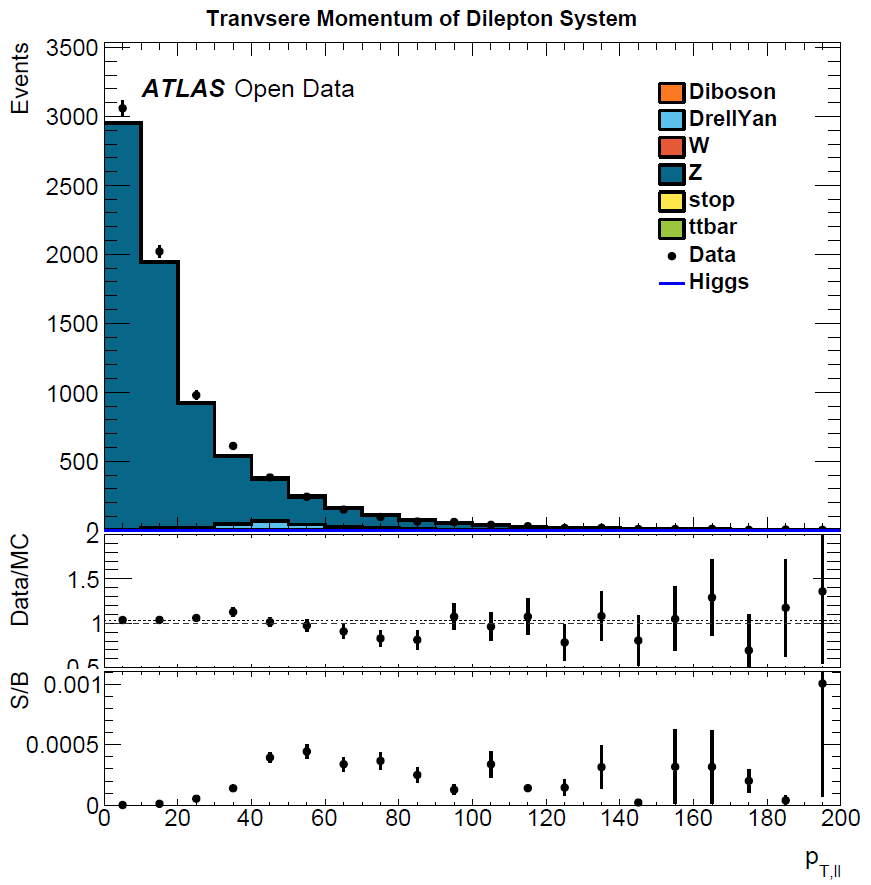
\includegraphics[width=.8\linewidth]{../Pictures/Auswertung/nocuts_momentum.png}
\caption{Daten ohne Cuts}
\end{subfigure}%
\begin{subfigure}{.5\textwidth}
\centering
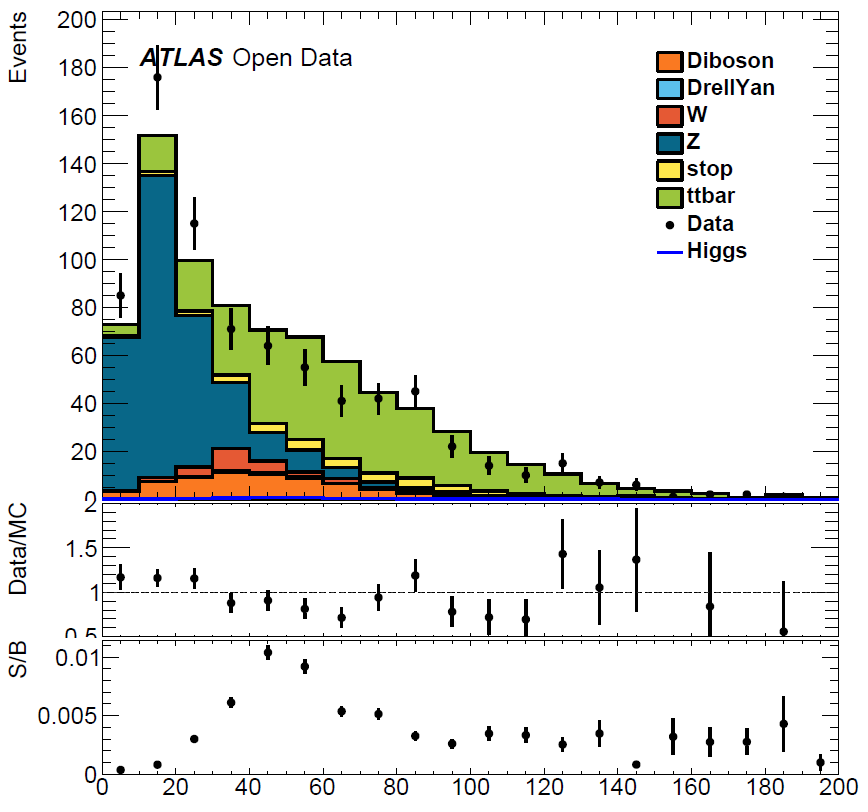
\includegraphics[width=.8\linewidth]{../Pictures/Auswertung/1cut_momentum.png}
\caption{Nur gemischte Leptonen und kein Ladungsüberschuss}
\end{subfigure}%
\vskip\baselineskip
\begin{subfigure}{.5\textwidth}
\centering
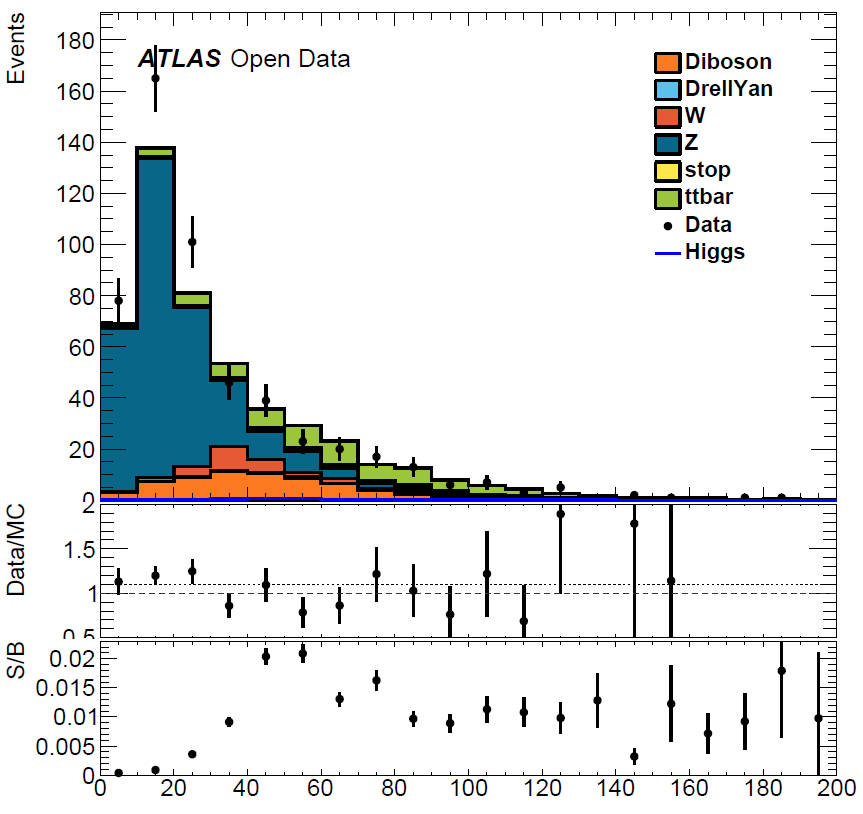
\includegraphics[width=.8\linewidth]{../Pictures/Auswertung/2cut_momentum.png}
\caption{Cut aller b-Jets}
\end{subfigure}%
\begin{subfigure}{.5\textwidth}
\centering
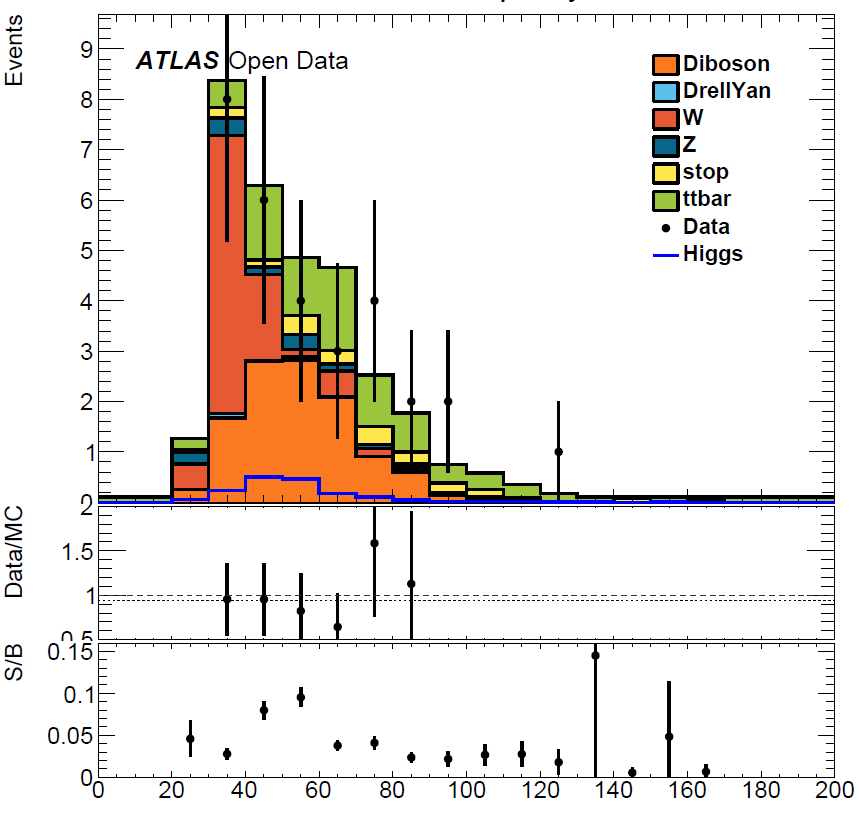
\includegraphics[width=.8\linewidth]{../Pictures/Auswertung/3cut_momentum.png}
\caption{weitere Cuts}
\end{subfigure}%
\caption{Auswirkungen der Cuts auf die Ereignisse unter Betrachtung des Leptonenimpulses}
\label{Cuts_momentum}
\end{figure}

Ausgehend von diesen Daten wurde nun zur statistischen Analyse der p-Value berechnet.
Für diese Berechnung wurden 10000 Pseudoexperimente durchgeführt.
Als Ergebnis ergaben sich ein p-Value von 0.0039 und eine obere Grenze für $\mu$ von 1.
Nach Konventionen der Teilchenphysik, ist ein p-Value von $5,7 \cdot 10^{-7}$ (entspricht $5 \sigma$) notwendig um von der Entdeckung eine Teilchens zu sprechen, dies ist hier offenbar nicht der Fall.
Ein p-Value von $0,05$ ($2 \sigma$) ist jedoch bereits ausreichend um die Nullhypothese, also die Nichtexistenz des Higgs-Bosons, zu verwerfen.
Dies ist hier offenbar der Fall, sodass wir davon ausgehen können, dass unsere Daten in guter Übereinstimmung mit dem Standardmodell mit Higgs-Boson sind.
